\section{Nhận dạng địa điểm trực quan - Visual Place Recognition}

Với mục đích trả lới câu hỏi: "Bức ảnh này được chụp ở đâu", nhận dạng địa điểm trực quan để xuất một hướng tiếp cận lấy cảm hướng từ bài toán truy xuất ảnh (Image Retrieval) \cite{2022arXiv220105816X}. Sử dụng mô hình truy xuất với một cơ sở dữ liệu linh hoạt (xem hình \ref{fig:ir}), hướng tiếp cận giúp bài toán định vị trực quan tăng cường đáng kể khả năng mở rộng về phạm vi mà không chịu quá nhiều tổn hại về hiệu năng. Đặt dưới ống kính giới hạn về loại dữ liệu có được, việc thu thập chỉ dữ liệu ảnh RGB, nhiều nghiên cứu trong lĩnh vực VPR đã đạt được nhiều thành tựu đáng kể. Mặc dù chưa thể vượt qua hiệu năng trong chất lượng định vị vị trí so với các hướng tiếp cận sử dụng dữ liệu RBG-D, các mô hình nghiên cứu đã phát triển phạm vi xử lý bài toán gấp bội, đạt mức độ linh hoạt và hiệu năng ổn định ở các tập dữ liệu cấp độ thành phố \cite{alibey2023mixvpr} và cấp độ thế giới \cite{keetha2023anyloc}. Vì lý do này, chúng tôi cho rằng hướng tiếp cận sử dụng mô hình VPR là hướng tiếp cận phù hợp và có tiềm năng nhất cho bài toán định vị trực quan trong môi trường đô thị.

\begin{figure}[H]
    \centering
    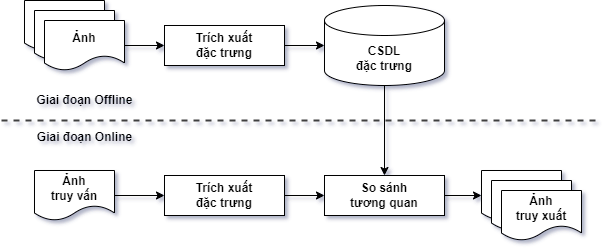
\includegraphics[width=0.8\textwidth]{pics/Chapter2/IR.drawio.png}
    \caption[Mô hình truy xuất ảnh cơ bản]{Mô hình truy xuất ảnh (Image retrieval) cơ bản.}
    \label{fig:ir}
\end{figure}

Các mô hình VPR thường được thiết kế để sử dụng một cơ sở dữ liệu hình ảnh đã được gắn nhãn với thông tin vị trí của thiết bị chụp. Sau khi truy xuất được ảnh, thông tin vị trí của ảnh truy xuất sẽ được xem là vị trí gần đúng cho hình truy vấn hoặc sẽ trở thành đặc trưng giúp mô hình tiếp tục tính vị trí chính xác của ảnh truy vấn. Tuy nhiên, quá trình truy xuất ảnh thông thường đạt kết quả rất kém khi được áp dụng trực tiếp cho quá trình nhận dạng địa điểm trực quan do các đặc trưng biểu diễn được khai phá đều tất cả các yếu tố xuất hiện trong ảnh. Những dữ liệu ảnh cho cùng một phong cảnh, mặt khác, lại chứa rất nhiều yếu tố che khuất, gây nhiễu, "đánh lạc hướng" quá trình khai thác (distractors) như sự hiện diện của cây cối, con người, động vật, phương tiện giao thông, cũng như sự khác biệt về chất lượng ánh sáng, thời gian, mùa màng. Đặc điểm này đã thúc đấy nghiên cứu của lĩnh vực để đề xuất các giải pháp để thích ứng bài toán truy xuất ảnh cho tập dữ liệu địa danh. Các lĩnh vực được tập trung phát triển có thể được tổng kết lại theo một quy trình ba bước \cite{Masone2021ASO}:

\begin{enumerate}
    \item bước trích xuất và mã hóa đặc trưng trích xuất một véc-tơ biểu diễn từ mỗi ảnh trong cơ sở dữ liệu để đại diện cho nội dung của ảnh (\textit{image representation});
    \item bước tìm kiếm tương đồng sử dụng các thuật toán so sánh tương đồng để đánh giá và tìm các ảnh trong cơ sở dữ liệu có nội dung tương tự nhất với ảnh truy vấn;
    \item bước hậu xử lý và lọc, sắp xếp và tinh chỉnh kết quả trả về từ bước tìm kiếm tương đồng, đưa ra kết quả cuối cùng.
\end{enumerate}

Tại đề mục này, chúng tôi sẽ mô tả quá trình phát triển, các phát hiện nền tảng và những hướng phát triển có tiềm năng cho bài toán nhận dạng địa điểm trực quan sử dụng dữ liệu ảnh ba kênh RGB.

\subsection{Trích xuất và biểu diễn đặc trưng}

Dưới góc nhìn một bài toán truy xuất ảnh, các đặc trưng biểu diễn của ảnh sẽ mang tính quyết định đối với chất lượng và hiệu năng của cả mô hình. Để đảm bảo khả năng biểu diễn tốt cho các đặc trưng ảnh ở các địa danh khác nhau, quá trình trích xuất đặc trưng, ban đầu, được thiết kế một cách thủ công, đến từ kiến thức chuyên môn. Các nghiên cứu bước đầu đặt ra các định nghĩa về các loại đặc trưng: đặc trưng lân cận, đặc trưng toàn cục và độ quan trọng của chúng. Thời gian gần đây, với sự phát triển của thị giác máy tính, các phương pháp học biểu diễn bằng mạng neuron học sâu đạt được các thành tựu nổi bật, đặc biệt là mạng neuron tích chập thay thế chức năng của đặc trưng thủ công.

\subsubsection{Biễu diễn đặc trưng lân cận - Local descriptors}

Trong bài toán học biễu diễn đặc trưng, một đặc trưng lân cận chỉ phân tích, biểu diễn ý nghĩa của một nhóm các điểm ảnh nhỏ và chỉ ra sự khác biệt giữa chúng với các nhóm các điểm ảnh lân cận \cite{CGV-017-localdescriptors}. Các nhóm điểm ảnh được tạo ra bằng cách chia mỗi hình ảnh thành lưới với độ phân giải nhất định và tất cả các nhóm điểm ảnh được thu thập, trích xuất để tìm đặc trưng. Để áp dụng cho bài toán truy xuất hình ảnh trực quan, các thuật toán lựa chọn như Hessian-Affine detector \cite{hessian-affine-detector}, MSER\cite{MSER-detector} được áp dụng để lựa chọn chỉ những nhóm điểm ảnh mang tính quan trọng, quyết định đến sự khác nhau giữa các ảnh và loại bỏ các nhóm điểm ảnh dễ bị ảnh hưởng bởi yếu tố môi trường. Vào thời gian đầu, việc truy xuất đặc trưng từ các nhóm ảnh, điểm ảnh được thực hiện bằng cách sử dụng các thuật toán như SIFT \cite{lowe1999object}, SURF \cite{bay2006surf}, RootSIFT \cite{Arandjelovi2012ThreeTE}, BRIEF \cite{brief}, DSP-SIFT \cite{Dong2014DomainsizePI} và đặc trưng kernel \cite{kernel-descriptors}. Các hướng tiếp cận mới hơn cho rằng các hướng tiếp cận trên sử dụng số lượng lớn đặc trưng cần trích xuất và lưu trữ trong khi không phải tất cả các đặc trưng đều có đủ tính phân biệt cho quá trình truy xuất ảnh \cite{predicting-good-features}, từ đó, đề xuất thêm quá trình lọc đặc trưng vào quá trình trích xuất. Năm 2014, Jégou và Zisserman chuẩn hóa quá trình trích xuất vector biểu diễn từ đặc trưng cục bộ thành quy trình 2 bước\cite{Jegou_2014_CVPR}:
\begin{enumerate}
    \item bước nhúng chuyển mỗi vector đặc trưng lên không gian mới có số chiều cao hơn,
    \item bước tổng hợp tạo chỉ một vector biểu diễn từ các vector đã tạo.
\end{enumerate}
Năm 2015, \cite{selective-match-kernel} đề xuất hàng loạt các phương án cho các bước nhúng, tổng hợp, cùng với các giải pháp để lựa chọn mức độ đóng góp của mỗi cặp biểu diễn cho một nhóm các ảnh, đánh dấu nền móng về hướng phát triển và hiện thực cho các mô hình học biễu diễn đặc trưng cục bộ sau này.

\subsubsection{Biễu diễn đặc trưng toàn cục  - Global descriptors}

Trong khi việc tổng hợp các vector biểu diễn cục bộ hỗ trợ việc truy xuất một vector biễu diễn cho một hình ảnh, các vector biểu diễn toàn cục có thể truy xuất tất cả thông tin này một cách trực tiếp. Khác với vector trích xuất cục bộ, các vector trích xuất toàn cục đọc và trích xuất biểu diễn đặc trưng cho toàn bộ bức ảnh và chỉ ra các đặc điểm khác biệt giữa bức ảnh này và bức ảnh khác. Việc truy xuất vector toàn cục có thể được hiện thực và thực thi với yêu cầu tài nguyên ít hơn sơ với việc truy xuất vector cục bộ, nhưng đồng thời cũng giảm đi khả năng phân biệt và tính bền bỉ trước các yếu tố thay đổi do điều kiện môi trường, góc chụp và các yếu tố bị che khuất. Mặc dù vậy, lợi ích của việc trích xuất đặc trưng cục bộ, áp dụng bởi các phương pháp như HOG \cite{HOG}, Gist \cite{GIST}, vẫn được xem trọng trong quá trình trích xuất biểu diễn đặc trưng toàn cục và trở thành cảm hứng cho các mô hình học biểu diễn sử dụng mạng neuron học sâu sau này.

\subsubsection{Học biễu diễn bằng mạng neuron học sâu tích chập và các lớp kết nối đầy đủ}

Với sự thành công của mạng neuron học sâu trong lĩnh vực thị giác máy tính\cite{krizhevsky2012imagenet}, các mô hình học sâu này đã được công nhận là những phương pháp tạo biểu diễn vô cùng hiệu quả. Đồng thời, một số bài báo cũng đã chỉ ra khả năng học đặc trưng thường thấy và chuyển tiếp được (transferable) đến các bài toán khác \cite{Oquab_2014_CVPR,ZeilerVisualizingAU,Chen2018DeepLabSI}.

\begin{figure}[h]
    \centering
    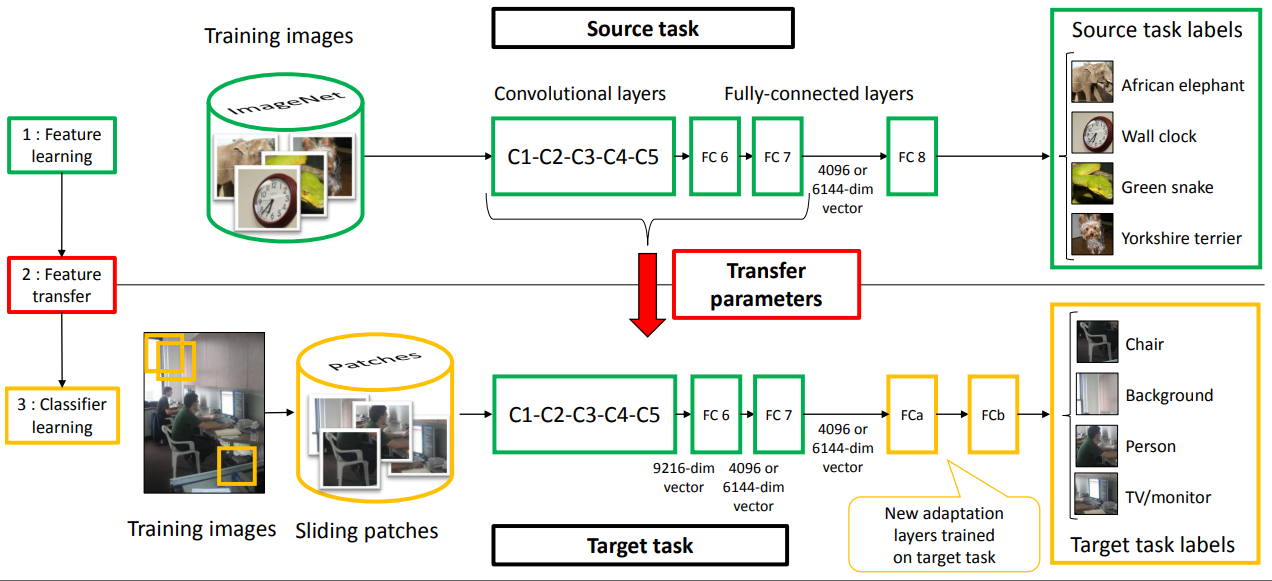
\includegraphics[width=\textwidth]{pics/Chapter2/cnn_transfer.png}
    \caption{Chuyển tiếp thông số của một mô hình mạng neuron học sâu tích chập\cite{Oquab_2014_CVPR}}
\end{figure}

Các mô hình học sâu tích chập đầu tiên được sử dụng cho bài toán truy xuất hình ảnh trực quan được cấu hình từ các lớp kết nối đầy đủ\cite{razavian2014cnn, gong2014multiscale, babenko2014neural, deepindex, image-classification-retrieval, wang2014deep} của một mạng phân loại, được huấn luyện trên tập dữ liệu ImageNet\cite{russakovsky2015imagenet}, đạt hiệu quả đáng kể khi sử dụng hàm mất mát triplet\cite{wang2014deep, gomezojeda2015training}. Tuy nhiên, có thể sớm nhận thấy rằng các mô hình sử dụng nhiều lớp kết nối đầy đủ có ý nghĩa tương ứng với các biểu diễn đặc trưng toàn cục. Các biểu diễn đặc trưng tạo ra được bằng cách sử dụng phương pháp này thiếu độ bền đối với dữ liệu chứa nhiều yếu tố gây nhiễu, che khuất và không đủ các yếu tố bất biến đối với biến thể tịnh tiến và tỉ lệ. Để khắc phục các hạn chế này, nhiều mô hình học sâu đã đề xuất các phương án cắt ảnh thành nhiều nhóm điểm ảnh và huấn luyện nhiều biểu diễn với kết nối đầy đủ cho mỗi hình \cite{razavian2014cnn, babenko2014neural}. Khi đánh giá các cách tiếp cận này so với các phương pháp trích xuất đặc trưng thủ công cục bộ, các mô hình học sâu sử dụng ít bộ nhớ hơn nhưng yêu cầu số lượng tính toán cao hơn. Các biểu diễn kết nối đầy đủ bị giới hạn bởi kích thước đầu vào cố định và lượng lớn các tham số.

\subsubsection{Học biểu diễn bằng mạng neuron tích chập}

Nỗ lực tìm giải pháp cho các giới hạn của mạng neuron kết nối đầy đủ đã trở thành cảm hứng cho các phương pháp sử dụng trực tiếp kết quả nhận được từ các lớp tích chập của mạng neuron học sâu. Áp dụng hướng tiếp cận đầu tiên chính là bài nghiên cứu của Babenko và nnk \cite{babenko2014neural}. Mạng neuron tích chập tạo ra một tenxơ (tensor) có cấu hình \(H \times W \times C\), trong đó \(C\) là số kênh, \(H\) và \(W\) là chiều cao và chiều rộng của ảnh. Babenko và nnk tạo ra vector biểu diễn bằng cách làm phẳng và chuẩn hóa lớp \(H \times W \times C\). Một số bài báo lấy cảm hứng từ hướng nghiên cứu này \cite{hou2015convolutional}, sau đó, đã thể hiện rằng vector biểu diễn mạng neuron học được, tùy vào phương án kết hợp lớp tenxơ, có thể mang ý nghĩa và chức năng tương tự với biểu diễn đặc trưng toàn cục trong khi tránh được các hạn chế của các mô hình học sâu sử dụng lớp kết nối đầy đủ. Các giải pháp này có thể được phân loại vào hai nhóm chính \cite{Masone2021ASO}:

\begin{itemize}
    \item gom cụm đặc trưng (feature aggregation) tích chập bằng các giải pháp lấy cảm hứng từ trích xuất đặc trưng thủ công cục bộ;
    \item tổng hợp đặc trưng (feature pooling) bằng cách khái quát hóa các đặc trưng tích chập.
\end{itemize}

\begin{figure}[h]
    \centering
    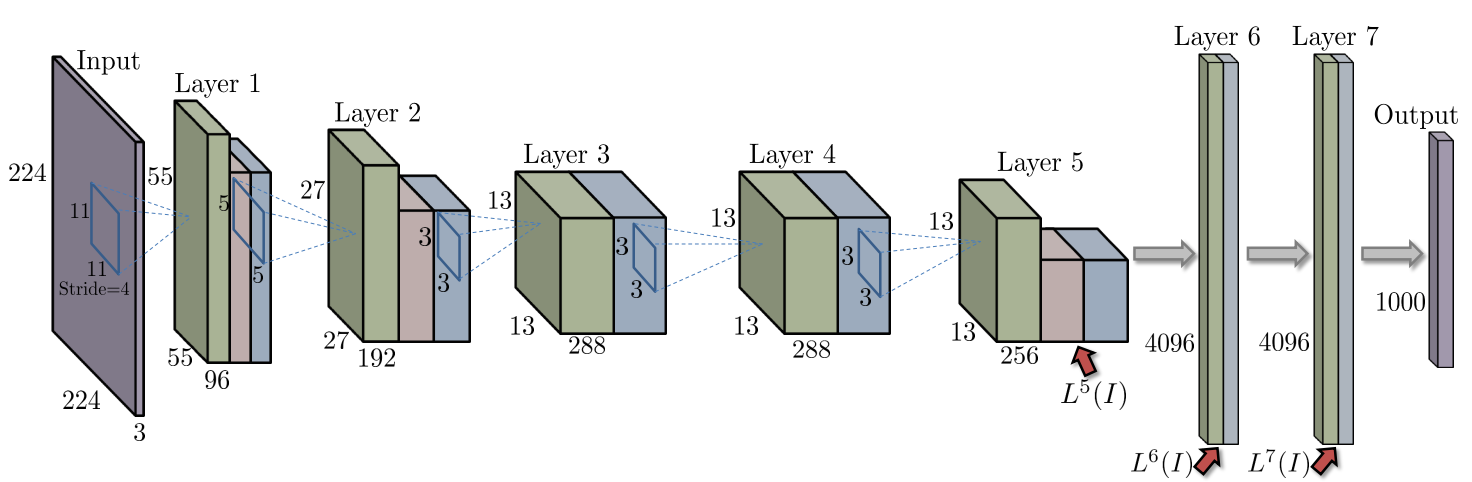
\includegraphics[width=\textwidth]{pics/Chapter2/firstcnns.png}
    \caption{Minh họa kiến trúc một mô hình CNN \cite{babenko2014neural}}
\end{figure}

Khi thực hiện gom đặc trưng trên lớp đặc trưng \(H \times W \times C\), lớp tích chập được đặt dưới góc nhìn là một lưới \(H \times W \) chứa các đặc trưng \(C\) chiều với mỗi đặc trưng là một vector có vùng nhận thức nhỏ. Bằng cách này, kết quả nhận được từ lớp tích chập có thể được đồng hóa (assimilated) thành một tập hợp các vector cục bộ được bố trí dày đặc. Tập hợp các vector dày đặc tiếp tục được mã hóa thành một vector biểu diễn và được sử dụng cho quá trình so sánh và truy xuất bằng các giải thuật so sánh tương đồng như khoảng cách Euclidean, tương đồng cosine. Sử dụng phương pháp này, việc mã hóa đặc trưng cho bước tìm kiếm tương đồng có thể áp dụng các hướng tiếp cận xử lý đặc trưng thủ công cục bộ như VLAD\cite{vlad}, BoW\cite{Mohedano_2016}, ASMK\cite{cao2020unifying}. Các nhà nghiên cứu tiếp tục đề xuất các phương pháp gom cụm có khả năng kết hợp trực tiếp với mạng neuron tích chập toàn bộ để cung cấp khả năng huấn luyện cả mô hình đầu-cuối \cite{ong2017siamese}. Đánh dấu một bước tiến quan trọng trong nỗ lực tìm giải pháp cho bài toán nhận diện địa điểm trực quan chính là lớp gom cụm NetVLAD \cite{arandjelovic2016netvlad}, hiện thực mô hình mã hóa và gom cụm VLAD với các phép tính khả vi cho phép mô hình khả năng huấn luyện đầu cuối một cách linh hoạt với nhiều tham số huấn luyện hơn so với VLAD thông thường. Hướng tiếp cận của các tác giả NetVLAD được tiếp tục hiện thực và sử dụng đến nay, đồng thời trở thành cảm hứng cho các hướng tiếp cận hiện đại hơn sau này.

\begin{figure}[h]
    \centering
    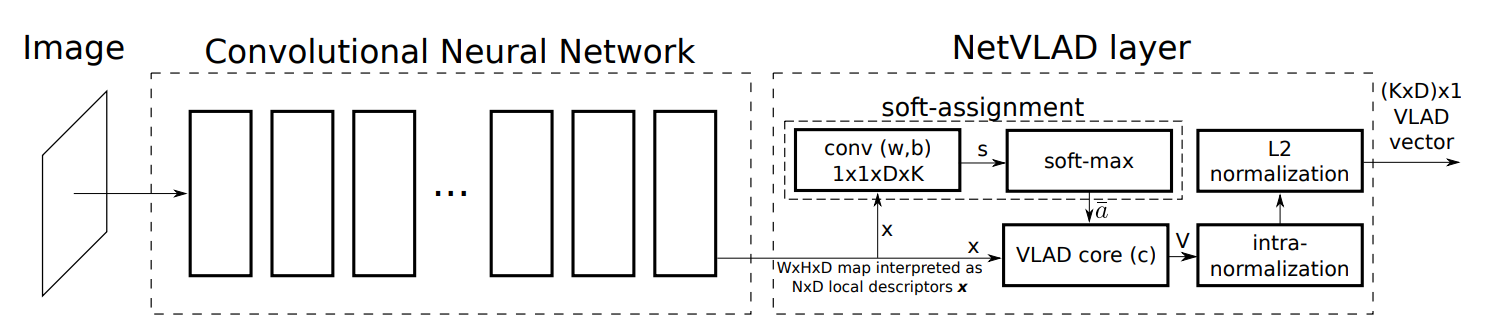
\includegraphics[width=\textwidth]{pics/Chapter2/netvladcnn.png}
    \caption{Minh họa kiến trúc một mô hình CNN được kết nối với lớp NetVLAD \cite{arandjelovic2016netvlad}}
\end{figure}

Tổng hợp đặc trưng lấy cảm hứng từ các nghiên cứu về mạng neuron tích chập. Các nhà nghiên cứu đã chỉ ra các đặc trưng từ những lớp tích chập giữa, cuối có tiềm năng được gom đặc trưng và sử dụng trực tiếp cho quá trình phân loại và tìm kiếm tương qua mà không cần mã hóa. Quá trình tổng hợp đặc trưng, tuy có thể được thực hiện một cách tương đối đơn giản như việc sử dụng một lớp max-pooling, lại truy xuất được các đặc trưng biểu diễn với số chiều thấp, mức chiếm dụng bộ nhớ thấp và hiệu năng vượt trội hơn so với đặc trưng biểu diễn được thiết kế thủ công. Các tác giả của bài báo \cite{mousavian2015deep} nhận thấy rằng phương pháp max-pooling có độ bền cao hơn đối với sự thay đổi về tỉ lệ trong khi sum-pooling có độ nhạy với các yếu tố gây nhiễu hơn. Họ kiểm thử một mô hình kết hợp cả hai phương pháp, SPoC, với mục đích đúc kết được điểm mạnh của cả hai phương pháp và đã đạt kết quả đáng kể. Tương tự, Tolias và những cộng sự \cite{tolias2015particular} phát triển quy trình mã hóa R-MAC (Regional Maximum Activations of Convolutions), tính toán vector max-pooling cho nhiều vùng ảnh khác nhau và tổng hợp chúng bằng lớp sum-pooling. R-MAC và SPoC là cảm hứng cho sự ra đời của GeM \cite{GeM} - lớp aggregation trung bình tổng quát. Áp dụng một tham số cho mỗi lớp đặc trưng và hiện thực lớp trung bình tổng quát dự trên các tham số đó, GeM đạt được hiệu quả vượt trội hơn cả R-MAC và SPoC và trở thành một trong những phương pháp tổng hợp đặc trưng hiệu quả nhất cho đến nay.

\subsection{Học nhận diện địa điểm trực quan}

Để đạt hiệu quả cao trong bài toán nhận diện địa điểm trực quan, ngoài việc truy xuất được các biểu diễn đặc trưng tốt, nhiều nghiên cứu còn tập trung phát triển quá trình học truy xuất, đặt quá trình huấn luyện mô hình dưới nhiều hướng tiếp cận khác nhau. Các hướng tiếp cận này có thể được chia thành hai nhóm chính: học truy xuất thông qua phân loại và học để xếp hạng. Ngoài ra, một số nghiên cứu còn tập trung vào khả năng học từ kiến thức chuyên môn hoặc tối ưu hóa quá trình học để xếp hạng với hàm mất mát lấy cảm hứng từ phương pháp xếp hạng danh sách (listwise ranking).

\subsubsection{Học truy xuất thông qua phân loại}

Vì bài toán phân loại là một trong những bài toán đầu tiên thể hiện kết quả tốt khi áp dụng mạng nơ-ron tích chập vào quá trình trích xuất đặc trưng, các mô hình học sâu tích chập được sử dụng cho bài toán nhận diện địa điểm trực quan đầu tiên lấy cảm hứng lớn từ các mô hình phân loại thay vì các mô hình truy xuất. Các mô hình này sử dụng một mạng nơ-ron tích chập đã được huấn luyện trên tập dữ liệu ImageNet \cite{krizhevsky2012imagenet}. Học truy xuất thông qua phân loại cho phép các nhà nghiên cứu huấn luyện được các véc-tơ đặc trưng toàn cục với kích thước nhỏ, sử dụng nhãn ở cấp độ ảnh mà không cần khai phá thông tin tương quan (example mining) trong quá trình huấn luyện, dẫn tới yêu cầu tài nguyên tính toán thấp hơn đáng kể so với các mô hình hiện tại, có tiềm năng lớn trong việc mở rộng phạm vi của bài toán truy xuất lên các tập dữ liệu lớn. Đảm nhận trách nhiệm trích xuất đặc trưng biểu diễn, một số đánh giá sơ bộ cho thấy các mô hình truy xuất thông qua phân loại, mặc dù đạt kết quả tốt trong bài toán phân loại các lớp ngữ nghĩa và nhận diện ảnh ở địa danh khác nhau, không đảm bảo sẽ học được các biểu diễn đặc trưng hiệu quả cho các yếu tổ thay đổi giữa các phần từ trong một lớp, quá trình so sánh tương quan và truy xuất từ cơ sở dữ liệu \cite{arandjelovic2016netvlad, gordo2016deep, randenovic2016BoW}, thúc đẩy các nhà nghiên cứu đến các hướng tiếp cận khác. Gần đây, sự phát triển của các giải pháp phân loại ở các bài toán trích xuất đặc trưng khác đã khơi dậy lại nỗ lực nghiên cứu phương pháp này với xu hướng tăng cường khả năng học các biểu diễn đặc trưng mang tính phân biệt tốt hơn cho những yếu tố thay đổi giữa các phần tử trong cùng một lớp. Nổi bật với hai bài báo \cite{cao2020unifying, yokoo2020twostage} sử dụng hàm mất mát ArcFace \cite{Deng_2022} và tương đồng cosine để huấn luyện mô hình truy xuất thông qua phân loại, đạt kết quả tốt hơn các phương pháp truy xuất thông qua phân loại trước đó. Lấy cảm hứng từ hàm mất mát ArcFace \cite{Deng_2022}, CosPlace \cite{berton2022rethinking} tiếp tục cải tiến phương pháp truy xuất thông qua phân loại, đạt kết quả tốt nhất hiện tại cho tập dữ liệu Tokyo 24/7(Recall@5) \cite{Torii-CVPR2015} và SF-XL \cite{berton2022rethinking}. Tiếp tục phát triển từ kết quả đạt được tại CosPlace \cite{berton2022rethinking}, Berton và nnk phát triển mô hình EigenPlaces \cite{berton2023eigenplaces} đạt kết quả tốt nhất hiện tại cho tập dữ liệu AmsterTime \cite{yildiz2022amstertime}, EynSham \cite{eynsham2009}, Pittsburgh-30k-test \cite{6618963}, San Francisco Landmark \cite{5995610}, SF-XL test v1 \cite{berton2022rethinking}, Tokyo247 \cite{Torii-CVPR2015}.

\begin{figure}[H]
    \centering
    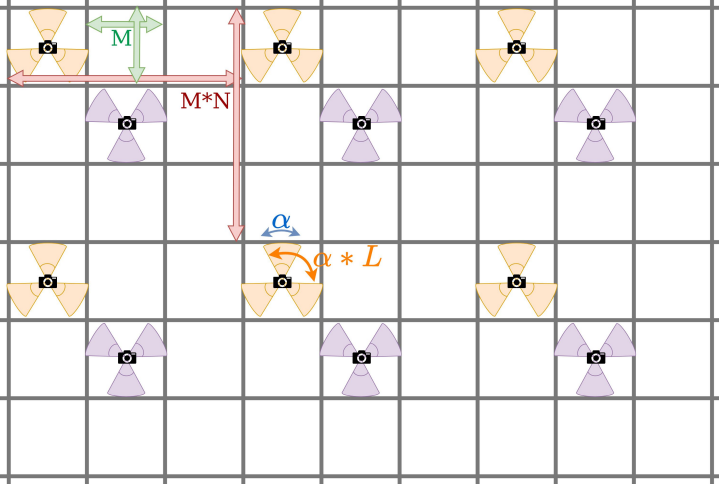
\includegraphics[width=0.7\textwidth]{pics/Chapter2/cosplaceclassify.png}
    \caption{Minh họa cách phân loại dữ liệu của mô hình CosPlace \cite{berton2022rethinking}}
\end{figure}

\subsubsection{Học truy xuất thông qua học xếp hạng}

Truy xuất hình ảnh, tương tự với bài toán "học xếp hạng", là quá trình học thông số và tìm phương thức truy xuất đặc trưng tốt nhất để biểu diễn sự tương quan giữa các phần tử trong tập dữ liệu dựa trên một hàm tính toán tương quan (distance function). Phần lớn các hướng tiếp cận cho bài toán nhận diện địa điểm trực quan sửa dụng một trong hai hàm mất mát chính với cùng ý tưởng:

\begin{itemize}
    \item hàm mất mát tương phản (contrastive loss), sử dụng các mạng nơ-ron siamese \cite{ong2017siamese, GeM, randenovic2016BoW}; và
    \item hàm mất mát ba phần tử (triplet loss), sử dụng các mạng nơ-ron có ba phần tử \cite{arandjelovic2016netvlad, gordo2016deep, gordo2017endtoend, wang2014learning, jin2017learned, zheng2018sift}.
\end{itemize}

Với mỗi mẫu dữ liệu huấn luyện, mô hình học truy xuất thông qua học xếp hạng được cung cấp những mẫu dữ liệu tích cực hoặc tiêu cực. Hàm mất mát có nhiệm vụ huấn luyện các đặc trưng sao cho những mẫu dữ liệu có giá trị tích cực sẽ có đặc trưng mang khoảng cách nhỏ và những mẫu dữ liệu có giá trị tiêu cực có khoảng cách lớn. Dưới góc nhìn của bài toán nhận diện địa điểm trực quan, một mẫu dữ liệu tích cực là ảnh ở cùng vị trí địa lý với ảnh huấn luyện, trong khi một mẫu dữ liệu tiêu cực là ảnh ở một vị trí địa lý khác. Các mô hình học truy xuất thông qua học xếp hạng có thể được chia thành hai nhóm chính: học truy xuất thông qua hàm mất mát tương phản và học truy xuất thông qua hàm mất mát ba phần tử. Như đã nhắc đến, để thực hiện quá trình học truy xuất thông qua học xếp hạng, các mô hình học truy xuất cần thực hiện quá trình khai phá thông tin tương quan (example mining) trong quá trình huấn luyện. Hướng tiếp cận này cho phép các nhà nghiên cứu phát triển các mô hình học giám sát yếu \cite{arandjelovic2016netvlad, jin2017learned} và học không giám sát \cite{radenovic2018fine} bằng cách lợi dụng các thông tin định vị để hỗ trợ quá trình khai phá. Tuy nhiên, quá trình khai phá này có chi phí tính toán cao, giới hạn thời gian và phạm vi dữ liệu có thể sử dụng để huấn luyện mô hình. \cite{arandjelovic2016netvlad} đánh dấu bước phát triển quan trọng trong hướng tiếp cận và đề xuất các hướng phát triển để tối ưu hóa quá trình này:

\begin{itemize}
    \item Lấy mẫu (Sampling): Hàm mất mát chỉ được tính cho tập hợp các mẫu dữ liệu tiêu cực và mỗi bước lấy mẫu sẽ thừa hưởng kết quả của những mẫu dữ liệu mang giá trị tiêu cực lớn nhất.
    \item Lưu đệm (Caching): Những đặc trưng được lưu trữ trong bộ nhớ đệm và chỉ được tính toán lại sau một số bước lấy mẫu huấn luyện nhất định tùy thuộc và tần suất học của mô hình (learning rate).
    \item Phân cụm (Clustering): Những đặc trưng được phân cụm dựa theo giá trị vị trí GPS thành các cụm nhỏ hơn và các mẫu huấn luyện trong cùng cụm sẽ chia sẻ cùng mẫu dữ liệu tiêu cực.
\end{itemize}


\subsection{Tìm kiếm tương đồng}
Bước thứ hai trong quy trình truy xuất ảnh thường là tác vụ tìm kiếm k lân cận gần nhất, hay nói là cách khác là tìm ra k ảnh có sự tương đồng cao nhất với ảnh nhận vào từ cơ sở dữ liệu. Tuy đơn giản về bản chất nhưng đây lại là tác vụ cực kỳ tốn kém về mặt tài nguyên đặc biệt là trong những bài toán với số chiều lớn. Một số nghiên cứu đã tăng tốc quá trình tìm kiếm bằng việc sử dụng các phương pháp tìm kiếm lân cận xấp xỉ (ANN) - không tiến hành quét cạn, sử dụng các kiến trúc chỉ mục khác,... \cite{4270175, Xie2015ImageCA, Mikolajczyk2007ImprovingDF, Muja2009FastAN, Muja2012FastMO, wang2017survey, magliani2019efficient, johnson2017billionscale}.

Với bước truy xuất ảnh, một yếu tố quan trọng cần cân nhắc chính là điều kiện bộ nhớ cần thiết của các phương pháp tìm kiếm - các biểu diễn ảnh quá lớn sẽ dẫn đến tiêu tốn cực nhiều tài nguyên của cơ sở dữ liệu. Để giải quyết vấn đề này, các nhà nghiên cứu có xu hướng hướng đến việc cải thiện tác vụ tìm kiếm tương đồng về mặt ổn định cũng như khả năng mở rộng. Các cấu trúc chỉ mục dựa trên tệp đảo ngược \cite{Salton1988TermWeightingAI} đã được sử dụng để thực hiện tìm kiếm không quét cạn, đặc biệt hiệu quả với các biểu diễn véc-tơ thưa \cite{Johns2011FromIT, Sivic2003VideoGA, imageSearchKernel, Mohedano2016sOL, noh2018largescale, Philbin2007ObjectRW}. Trong \cite{Johns2011FromIT}, thời gian truy xuất được giảm bằng cách nhóm các hình ảnh cơ sở dữ liệu tương tự và sau đó thực hiện việc ghép tương đồng theo cụm. Các kỹ thuật lượng tử hóa như k-means \cite{Philbin2007ObjectRW, Torii2013VisualPR}, nhị phân hóa \cite{Perronnin2010LargescaleIR} và lượng tử hóa tích \cite{imageSearchKernel} cũng được áp dụng để giảm yêu cầu bộ nhớ lưu trữ dữ liệu, các kỹ thuật này còn được kết hợp với tính toán khoảng cách không đối xứng \cite{5432202} và phép gán bội \cite{imageSearchKernel, Jgou2008HammingEA, 5432202, Philbin2007ObjectRW, Tolias2014VisualQE, Li2015PairwiseGM} để giảm thiểu tối đa lỗi lượng tử hóa. Kỹ thuật chỉ mục đảo cũng đã được tổng quát hóa để làm việc với lượng tử hóa tích \cite{Guo2016DeepLF, 5432202, Babenko2012TheIM}, cải thiện thêm tốc độ và độ chính xác của phép tìm kiếm, với một chi phí bộ nhớ tương đối nhỏ.

\subsection{Các mô hình truy xuất địa danh khác}
Các phương pháp nhận diện địa điểm trực quan thường được nghiên cứu theo xu hướng sử dụng ngữ cảnh của các ảnh trên đường phố. Việc có quyền truy xuất vào ảnh vệ tinh cũng như sự khuếch tán của rô-bốt trên không được trang bị camera đã mở ra một hướng phát triển mới. Một mặt, ảnh vệ tinh cho phép chúng ta có được đa dạng các góc nhìn cũng như một góc nhìn rộng hơn của khu vực. Mặt khác, chúng mở ra những thách thức như thiếu sót chi tiết trực quan.

\subsubsection{Định danh từ xa}
Trong truy xuất ảnh định danh từ xa, cũng như trong các tác vụ VPR cổ điển, mục đích vẫn là xác định vị trí ảnh nhận vào thông qua việc truy xuất ảnh tương đồng từ cơ sở dữ liệu. Do ảnh được chụp từ máy ảnh hướng xuống được trang bị trên một thiết bị bay hoặc từ vệ tinh dẫn đến việc ảnh sẽ phản ánh một khu vực địa lý lớn với nhiều vật thể có kích thước khác nhau. Các yếu tố vật thể dễ phân biệt ở tầng mặt đất như các tòa nhà lại không mang nhiều thông tin khi nhìn từ phía trên cao. Mặt khác, các yếu tố không mang quá nhiều thông tin hữu ích ở tầng mặt đất như đường xá lại quan trọng trong tác vụ định danh từ xa.

Dù cho có nhiều sự bất tương đồng, đã có những phương pháp VPR cổ điển được áp dụng để giải quyết bài toán định danh từ xa. Trong \cite{Tang2018UnsupervisedDF}, tác giả đề xuất sử dụng một phương pháp dựa trên túi-từ. Đầu tiên, các hình ảnh được chia thành các phân vùng sử dụng các phương pháp khác nhau. Sau đó, biểu diễn hình ảnh được xây dựng bằng cách kết hợp các đặc trưng ngầm được trích xuất bằng cách đưa mỗi phân vùng qua phần mã hóa của một mạng tích chập học sâu. Cuối cùng, túi-từ được tạo ra bằng cách sử dụng những biểu diễn này. Thay vì sử dụng phân vùng - tốn kém về mặt tài nguyên tính toán, \cite{Imbriaco_2019} đề xuất sử dụng kiến trúc DELF để trích xuất các đặc trưng cục bộ đáng chú ý sau đó kết hợp chúng thông qua trình tổng hợp VLAD. Ngoài ra, vì xác minh hình học khó áp dụng cho hình ảnh định dạng từ xa, các nhà nghiên cứu sử dụng mở rộng truy vấn dựa trên vector bộ nhớ \cite{7870636} để cải thiện kết quả truy vấn.

\begin{figure}[H]
    \centering
    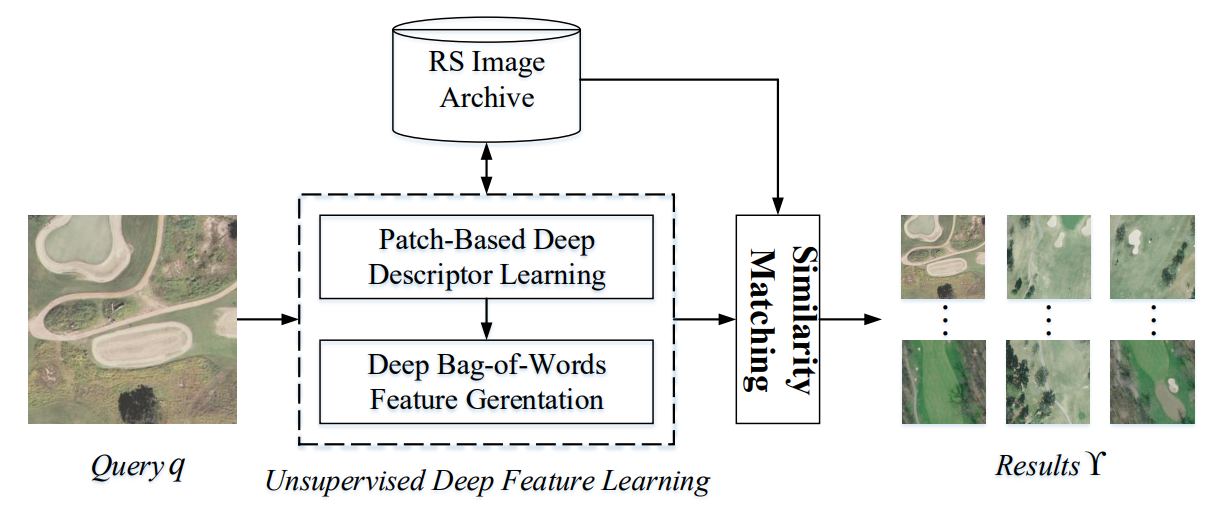
\includegraphics[width=\textwidth]{pics/Chapter2/rsir.png}
    \caption{Minh họa mô hình DBOW \cite{Tang2018UnsupervisedDF}}
\end{figure}

\subsubsection{Truy xuất vị trí từ các góc nhìn chéo (cross-view geo-localization)}
Một công dụng khác của ảnh trên không được sử dụng trong nhận diện địa điểm trực quan là truy xuất vị trí từ các góc nhìn chéo. Cụ thể với hướng tiếp cận này, ảnh nhận vào sẽ ở mức độ mặt đất và ảnh từ cơ sở dữ liệu sẽ là ảnh trên không. \cite{Lin2015LearningDR} xem xét trường hợp cụ thể trong đó các hình ảnh trên không được lấy từ cơ sở dữ liệu Google Street View và được chụp với góc khoảng 45 độ cùng với bản đồ độ sâu thô. Thông tin này, cùng với giả định của mô hình máy ảnh trực giao, cho phép chiếu lại các hình ảnh tầng mặt đất lên tầng trên không và thiết lập các kết nối mặt đất-trên không. Những kết nối này sau đó được sử dụng như các mẩu dữ liệu để đào tạo một bộ trích xuất đặc trưng dựa trên CNN với mất mát đối lập. \cite{workman2015widearea} đề xuất huấn luyện một mô hình nơ-ron tích chập để trích xuất biểu diễn kết nối đầy đủ của các hình ảnh trên không bằng cách sử dụng một hàm mất mát $l_2$ để căn chỉnh những biểu diễn này với những biểu diễn được trích xuất từ mô hình đã được huấn luyện trước cho các hình ảnh mặt đất tương ứng. Góc nhìn chéo cũng được tận dụng trong \cite{Castaldo2015SemanticCM} cho trường hợp của hình ảnh hệ thống thông tin địa lý gắn với bản đồ ngữ nghĩa. Tương tự như \cite{Lin2015LearningDR}, một phép chiếu lại được sử dụng để chỉnh sửa hình ảnh tầng mặt đất, nhưng phép chiếu lại được áp dụng cho một bản sao có được phân chia ngữ nghĩa của ảnh truy vấn.

\begin{figure}[H]
    \centering
    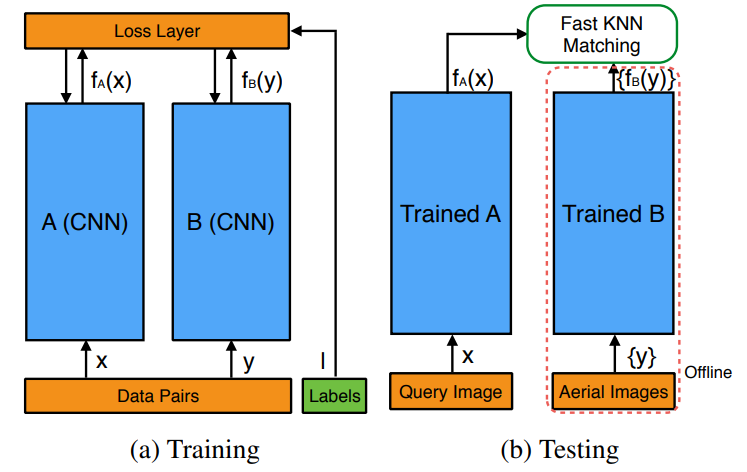
\includegraphics[width=\textwidth]{pics/Chapter2/wherecnn.png}
    \caption{Minh họa mô hình DBOW \cite{Lin2015LearningDR}}
\end{figure}

\subsection{Các khó khăn so với bài toán truy xuất hình ảnh cơ bản}

Mặc dù bài toán truy xuất địa danh thường được đánh giá và phát triển dưới góc nhìn là một bài toán truy xuất hình ảnh hoặc truy xuất instance, để biến đổi các giải pháp cho bài toán truy xuất hình ảnh thành giải pháp cho bài toán này, chúng ta cần phải đề xuất các hướng phát triển để triệt tiêu các khó khăn gắn liền với bản chất của dữ liệu địa danh. Khi nhận diện dữ liệu địa danh trong tập dữ liệu huấn luyện thành thị, mô hình học sâu sẽ phải xử lý một lượng lớn dữ liệu chứa các yếu tố lặp đi lặp lại đến từ kiến trúc nhân tạo như đường phố và cơ sở hạ tầng. Khi xử lý dữ liệu được thu thập trong một khoảng thời gian dài, mô hình học sâu cần đảm bảo tính bền của các đặc trưng biểu diễn trước các yếu tố thay đổi về điều kiện môi trường và phông cảnh được tạo ra do nhiều yếu tố phức tạp như mùa màng, thời tiết, thời gian, ánh sáng, \dots. Ngoài ra, dữ liệu đại diện cho các đối tượng địa danh mà mô hình cần học thường được thu thập từ các góc nhìn khác nhau với thiết bị và cảm biến khác nhau, yêu cầu khả năng khái quát hóa cao của mô hình học sâu. Quá trình phát triển để tăng cường độ bền của đặc trưng biểu diễn trước thay đổi trong điều kiện tự nhiên, môi trường, xã hội, thiết bị thu thập dữ liệu đã đặt bài toán truy xuất địa danh vào một phân loại khác biệt so với bài toán truy xuất hình ảnh cơ bản. Trong phần này, chúng tôi sẽ trình bày các khó khăn đặc trưng của bài toán truy xuất địa danh và các hướng phát triển để giải quyết các khó khăn này, lấy cảm hứng từ các giải pháp đã được đề xuất cho bài toán truy xuất hình ảnh cơ bản và các bài toán khác.

\subsubsection{Chọn vật thể và góc nhìn}

Tập dữ liệu hình ảnh địa danh cần xử lý trong bài toán truy xuất địa danh mang nhiều yếu tố lộn xộn (clutter), gây nhiễu, tạo ra hiện tượng phân tâm (visual distractors) cho các mô hình. Từ những ngày đầu phát triển, các nhà nghiên cứu đã ghi nhận mức độ quan trọng của quá trình quan sát và chọn ra các thành phần, góc nhìn của ảnh mang giá trị thông tin cao và tránh các yếu tố gây nhiễu, giảm hiệu năng\cite{4270175, knopp2010avoiding, predicting-good-features, Torii2013VisualPR, arandjelovic2015dislocation}. Đến nay, các hướng tiếp cận thường tối ưu hóa quá trình này theo hai chiến lược chính:

\begin{enumerate}
    \item Chọn vùng (region selection)
    \item Cơ chế tập trung (attention) và lớp trọng số (weighting)
\end{enumerate}

Chọn vùng là một chiến lược để xử lý vấn đề cluterring và visual distractors. Bằng cách chọn ra các vùng trong ảnh mang giá trị thông tin cao, mô hình truy xuất so sánh tương quan giữa các đặc trưng biểu diễn trích xuất được từ các vùng khác nhau thay vì giữa các ảnh khác nhau, trên lý thuyết, dẫn đến hiệu năng cao và tính bền bỉ cho mô hình. Trên thực tế, tuy đạt được độ bền cao so với thay đổi về tỉ lệ và thay đổi góc nhìn, việc trích xuất các vùng ảnh trực tiếp từ ảnh đầu vào được đánh giá là kém hiệu quả và tốn nhiều tài nguyên tính toán. Một hướng tiếp cận khác sử dụng mạng học sâu tích chập, chia ảnh đầu vào bằng một lưới với kích thước cố định và trích xuất vùng ảnh từ các đặc trưng trích xuất được\cite{razavian2016visual, tolias2015particular}. Phướng tiếp cận này làm giảm được số lượng tham số cần học, tuy nhiên không giải quyết được vấn đề đã nhắc đến một cách hiệu quả. Kích thước lưới được quyết định một cách cố định và mà không tận dụng được bối cảnh của ảnh, dẫn đến số lượng các vùng ảnh được chọn không mang ý nghĩa tương đương với các vùng ảnh mang ý nghĩa bất kể độ mịn của lưới. Đồng thời, việc tăng độ mịn của lưới với mục tiêu tăng cường độ bền của mô hình sẽ làm tăng đáng kể số lượng các vùng ảnh được trích xuất, dẫn đến tăng đáng kể thời gian tính toán và số lượng tham số cần học, cho thấy rằng đây không phải là một hướng tiếp cận thân thiện với phạm vi lớn. Đề xuất các hướng giải quyết cho vấn đề này, các mô hình R-MAC\cite{tolias2015particular} được chỉnh sửa với các mạng đề xuất vùng tương tự với hướng tiếp cận được đề xuất trong Faster R-CNN\cite{ren2015faster} và mô hình ASMK aggregation\cite{selective-match-kernel} với cơ chế truy xuất sử dụng MobileNet V2\cite{sandler2018mobilenetv2, teichmann2019detect}. Ngoài ra, nhận thấy các lớp gần cuối của mạng học sâu tích chập thường thể hiện các đặc trưng ngữ nghĩa có ý nghĩa\cite{ZeilerVisualizingAU}, các hướng tiếp cận hiện đại thường khai thác trực tiếp đặc trưng từ các lớp sau của mạng tích chập cho tác vụ chọn vùng\cite{chen2017only, khaliq2019holistic}.

Cơ chế attention và lớp trọng số là một chiến lược mới, với mục tiêu chọn ra những thông tin, đặc trưng mang tính tương quan cao từ các hình ảnh để tăng hiệu năng hoạt động của các mô hình truy xuất địa danh. Khác với cơ chế chọn vùng, cơ chế attention không truy xuất thông tin từ những vùng mà mô hình cho là quan trọng, mà truy xuất tất cả các vùng trong ảnh cùng một lúc. Sau đó, các đặc trưng trích xuất được được tổng hợp lại dựa theo một lớp trọng số và điều kiện đánh giá cụ thể. Điều kiện đánh giá này, vào những ngày đầu, được thiết kế dựa theo các cơ chế phỏng đoán (heuristic) như khoảng cách so với trọng tâm hình ảnh, độ nổi bật của đặc trưng trong tất cả các kênh (channel), \dots. Hướng tiếp cận này đạt nhiều thành công trong các tập dữ liệu chứa các đối tượng lặp đi lặp lại và thiếu tính tương phản cao. Ngoài ra, sự đa dạng trong phương thức thiết kế lớp trọng số cho phép nhà nghiên cứu tùy chỉnh mô hình để giải quyết các vấn đề cụ thể. Tuy nhiên, các mô hình này dễ trở nên thiếu linh hoạt, khó huấn luyện để tổng quát hóa và chỉ đạt kết quả tốt nhất khi được huấn luyện đầu-cuối (end-to-end). Ngày nay, hướng tiếp cận này thường được hiện thực sử dụng cơ chế Transformers (một loại mô hình auto-encoder), Vision Transformers (ViT)\cite{dosovitskiy2020image}, \cite{shavit2023coarse}. Nhận thấy tác động tài nguyên của ViT, \cite{alibey2023mixvpr} đề xuất sử dụng mạng học sâu MLP-Mixer\cite{tolstikhin2021mlpmixer}, một mạng học sâu sử dụng nhiều lớp MLP (Multi-Layer Perceptron) kết nối đầy đủ (fully-connected) với nhau, để thay thế cho ViT với mục tiêu đạt được cùng hiệu năng nhưng đòi hỏi ít tài nguyên hơn. Tác giá của \cite{alibey2023mixvpr} cho rằng, cho tác vụ truy xuất địa danh, MLP-Mixer là một lựa chọn có tiềm năng cao để thay thế cho ViT.

\subsubsection{Góc nhìn ảo và sự biến dạng}

Trong thực tế, các đặc trưng cục bộ dày đặc được sử dụng cho quá trình so sánh tương quan, mặc dù mạnh mẽ hơn so với các đặc trưng cục bộ thưa thớt trước các thay đổi về ánh sáng \cite{zhou2016evaluating}, không thu hẹp được các ảnh hướng đến từ biến đổi hình học (tỷ lệ và góc nhìn). Đối mặt với vấn đề này, một số bài báo \cite{torii201524, taira2018inloc} đề xuất các chiến thuật sinh góc nhìn (view synthesis). Dựa vào cơ sở dữ liệu chứa ảnh RGB và thông tin độ sâu, các mô hình này truy xuất một danh sách các ví trí sơ bộ gần đúng và chế tạo góc nhìn ảo tương ứng, đưa ảnh truy vẫn và ảnh truy xuất về cùng một góc nhìn. Quá trình lựa chọn ảnh khớp tốt nhất được thực hiện một cách đơn giản, trực tiếp lên số lượng các điểm ảnh trùng và không trùng của các ảnh. Mặc dù hướng tiếp cận này tạo ra số lượng lớn các dị vật trong ảnh (visual artifacts), chiến thuật này thường đạt kết quả tốt hơn so với các mô hình truy xuất địa danh cơ bản.

Ngoài ra, trong các ứng dụng đặc biệt hơn như truy xuất vị trí từ các góc nhìn chéo, các mô hình cần phải truy vấn ảnh lấy được từ các góc nhìn trên không để so sánh với ảnh lấy được từ góc nhìn trên mặt đất và ngược lại. Sự khác nhau rất lớn về góc nhìn này đã tạo nên không ít khó khăn. Một giải pháp cho vấn đề này là quá trình chiếu tất cả các ảnh về một góc nhìn chung \cite{lin2015learning, castaldo2015semantic}. Một giải pháp khác sử dụng thêm các đặc trưng chỉ hướng (rolling descriptor) cho quá trình truy vấn để mã hóa thông tin chỉ hướng vào đặc trưng biểu diễn của các ảnh trong cơ sở dữ liệu \cite{xia2023convolutional}. Trong quá trình suy luận (inference), mô hình này khai phá thông tin chỉ hướng từ các ảnh góc rộng (panorama) để mã hóa vào biểu diễn truy vấn, so sánh tương quan giữa các đặc trưng biểu diễn này với các đặc trưng biểu diễn của các ảnh trong cơ sở dữ liệu.

\subsubsection{Thông tin ngữ nghĩa}

Việc thu thập và sử dụng thông tin ngữ nghĩa được đánh giá rất cao trong các hướng tiếp cận của bài toán. Thông tin này hỗ trợ trực tiếp quá trình chọn vùng và các điểm ảnh quan trọng như một yếu tố heuristic, cho phép các mô hình phát triển độ bền vững của mình trước các tác động môi trường và thay đổi trong điều kiện khách quan. Các hướng tiếp cận hiện đại ngay nay thường sử dụng triệt để mọi thông tin mà môi trường truy xuất cung cấp như thông tin về độ sâu, thông tin về mùa màng, thời gian, ánh sáng, \dots Ngoài ra, các loại thông tin như độ liên quan giữa số lượng, sự hiện diện của các phương tiện giao thông, các kiến trúc lặp đi lặp lại cũng hỗ trợ đáng kể cho quá trình lọc đặc trưng, loại bỏ các yếu tố gây nhiễu, lựa chọn các cột mốc địa danh có tính tương quan cao.

\subsubsection{Thông tin về độ sâu}

Thông tin độ sâu thường được xem là dữ liệu đi kèm với các tập dữ liệu truy xuất địa danh. Đóng vai trò là cầu nối giữa hình ảnh hai chiều và thông tin ba chiều của địa danh, thông tin độ sâu thường được sử dụng để tăng độ bền cho các mô hình học sâu trước các thay đổi về điều kiện ảnh. Ngoài ra, độ sâu còn có thể được tích hợp vào các đặc trưng biểu diễn để hỗ trợ quá trình trích xuất biểu diễn toàn cục cho quá trình truy xuất hình ảnh. Tuy nhiên, giống với các mô hình học từ dữ liệu thu thập được từ cảm biến độ sâu như LiDAR, việc đòi hỏi dữ liệu huấn luyện chứa thông tin về độ sâu là một hạn chế lớn, giảm khả năng mở rộng cho tập dữ liệu vì các vấn đề thu thập, lưu trữ, cập nhật và huấn luyện. Vì lý do này, một số hướng tiếp cận trong bài toán thường thiết kế các mô đun học sâu phụ cho mô hình của mình, với mục đích tự xây dựng lại một phiên bản cơ bản hơn của thông tin này trong quá trình huấn luyện. Sử dụng phương pháp tiếp cận này, mô hình chỉ cần nhận vào ảnh 2 chiều RGB trong quá trình truy xuất\cite{piasco2019learning}.

\subsubsection{Thích nghi với điều kiện môi trường thay đổi}

Những thách thức mà các mô hình truy xuất địa danh phải đối mặt khi đối mặt với các thay đổi về điều kiện môi trường như ánh sáng, thời tiết và mùa màng được công nhận rộng rãi\cite{zaffar2019levelling} và vẫn còn đươc xem là một vấn đề mở. Một lượng lớn các tài liệu nghiên cứu đã nghiên cứu các hạn chế của các đặc trưng học sâu trong các điều kiện khó khăn \cite{zhou2016evaluating, sunderhauf2015performance, chen2017deep} và các phân tích này đã cung cấp một số hướng dẫn để tìm ra các đặc trưng mạnh mẽ hơn. Các nhà nghiên cứu cho rằng, các đặc trưng cục bộ cần phải được phân bố một cách dày đặc mới có thể tránh khỏi vấn đề hiệu năng kém trước các thay đổi về độ sáng (ngày/đêm). Đồng thời, một giải pháp thay thế hiệu quả là quá trình tiền xử lý dữ liệu ảnh đầu vào bằng một mô hình học sâu đơn giản, với mục tiêu chuẩn hóa độ sáng của ảnh. Một số đánh giá xếp hạng cho thấy, các đặc trưng học sâu có hiệu năng tốt hơn trước khi được so sánh với các đặc trưng được thiết kế thủ công\cite{arandjelovic2017netvlad}. \cite{taira2018inloc} ghi nhận rằng đặc trưng cục bộ dày đặc hoạt động tốt trong môi trường trong nhà, nơi thiếu các đặc trưng lặp đi lặp lại và đặc trưng bề mặt vật liệu (texture) trong khi các mô đun trích xuất đặc trưng (feature extractions) hoạt động tốt hơn trong môi trường ngoài trời, khai thác các yếu tố ít thay đổi như kiến trúc và đặc điểm của đường phố. Một số hướng phát triển có tiềm năng sử dụng các mô hình có cơ chế tập trung lên những phần nhỏ của một ảnh như \cite{sunderhauf2015place, chen2017only, khaliq2019holistic} sử dụng chiến thuật vùng hấp dẫn (regions of interest), \cite{zhu2018attention, chen2017only, khaliq2019holistic, wang2019atloc, wang2022transvpr, alibey2023mixvpr} sử dụng cơ chế attention, \cite{garg2018lost, naseer2017semantics, seymour2019semantically}. Đồng thơi, sử dụng một chuỗi các hình ảnh liên tực thay cho một hình ảnh đơn lẻ cũng có tác động lớn đối với độ bền của mô hình trước điều kiện mô hình thay đổi \cite{naseer2018robust, hausler2019multi, hong2019textplace, chancan2020hybrid}.

Các giải pháp cho vấn đề thay đổi điệu kiện môi trường thường phải sử dụng các chiến thuật có yêu cầu tài nguyên lớn, khó phát triển quy mô. \cite{doan2019scalable} đề xuất một giải pháp ba bước để khắc phục các vấn đề này: xây dựng mô hình chứa cơ sở dữ liệu có thể tiếp tục mở rộng phạm vi với nhiều ảnh được thu thập ở các điều kiện môi trường khác nhau. Doan và nnk đề xuất mô hình:

\begin{enumerate}
    \item Một thuật toán nhận diện địa điểm trực quan được xây dựng dựa trên mô hình Markov ẩn (Hidden Markov Model) với hiệu năng huấn luyện và kiểm thử cao.
    \item Một chiến thuật chọn lọc điều chỉnh số lượng ảnh được thêm vào cơ sở dữ liệu, đảm bảo chỉ thêm các ảnh biểu diễn các ảnh với dữ liệu mới và chứa nhiều đặc điểm quan trọng.
    \item Một thuật toán nén hợp nhất các phần kết nối được với nhau trong cơ sở dữ liệu, giảm kích thước lưu trữ.
\end{enumerate}

Gần đây hơn, một số nghiên cứu tìm cách đối mặt với vấn đề này dưới góc nhìn khác, giải quyết vấn đề miền chéo, khi ảnh truy vấn chứa nhiều sự khác biệt về độ sáng, thời tiết, mùa màng hoặc thiết bị thu thập ảnh so với ảnh trong cơ sở dữ liệu. Hướng tiếp cận này đặt ra mục tiêu sinh ra ảnh mới để thay thế ảnh truy vấn, cùng mô tả một cảnh nhưng với với miền của ảnh trong cơ sở dữ liệu. Trong \cite{Porav2018AdversarialTF, Annosheh2019Night} quá trình sinh ảnh thường được thực hiện bởi mạng đối nghịch tạo sinh (GAN). Thay vì căn chỉnh dữ liệu các miền khác nhau, một hướng tiếp cận khác đặt trọng tâm trong quá trình học đặc trưng đa miền và tách cụm những đặc trưng phụ thuộc vào điều kiện môi trường và những đặc trưng bất biến \cite{yin2019multi}. Mạng đối nghịch tạo sinh đạt hiệu quả đáng kể đối với các vấn đề miền chéo chứa sự khác biệt về độ sáng, thời tiết hoặc mùa màng nhưng chưa giải quyết được vấn đề miền chéo chứa sự khác biệt về thiết bị thu thập. Trong thực tế, các tập dữ liệu huấn luyện mô hình luôn được thu thập trong khoảng thời gian sớm hơn so với dữ liệu truy vấn. \cite{wang2019attention} đề xuất kiến trúc sử dụng một mô hình trích xuất đặc trưng học sâu tích chập với lớp aggregation VLAD \cite{jegou2010aggregating} và hai mô đun chủ chốt:

\begin{itemize}
    \item một mô đun attention đánh giá độ quan trọng của các đặc trưng tổng hợp được từ lớp VLAD, và
    \item một hàm mất mát thích nghi miền sử dụng hàm khác biệt trung bình tối đa đa hạt nhân (multi-kernel maximum mean discrepancy hoặc MK-MMD) hỗ trợ mạng học được không gian chung của mà cả hai miền.
\end{itemize}

Trong đó, mô đun attention được đánh giá có cống hiến ít so với cải tiến chung của mô hình trong khi hàm mất mát nắm vị trí trọng tâm.

Thêm vào đó, đặt vấn đề dưới góc nhìn là quá trình thu thập dữ liệu, \cite{hu2020dasgil} đề xuất sử dụng tập dữ liệu ảo chứa thông tin độ sâu và thông tin ngữ nghĩa để huấn luyện mô hình học sâu. Quá trình huấn luyện lấy cảm hứng từ mô hình đối nghịch đảm bảo đặc trưng trích xuất được từ miền ảo và miền ảnh thật có độ phân bố tương tự nhau.

Trong [Adaptiveattentive geolocalization from few queries: A hybrid approach], Berton và nnk chứng minh hướng tiếp cận áp dụng kết hợp cả bài toán sinh dữ liệu (generative) và bài toán thích ứng miền (domain adaptation) có khả năng tăng hiệu năng của các mô hình cao.


\subsection{Phân tích và tổng hợp}

Trước sự phát triển của mạng học sâu tích chập trong lĩnh vực thị giác máy tính và hiệu năng của các đặc trưng toàn cục huấn luyện được, có thể nhận định rằng: trong tương lai, bài toán nhận diện địa điểm trực quan sẽ tiếp tục được phát triển với học biểu diễn đặc trưng toàn cục là chính và sẽ kết hợp với quá trình khai phá mối quan hệ cục bộ giữa các đặc trưng. Hướng phát triển này cho phép các nhà nghiên cứu huấn luyện và chạy mô hình với tác động tài nguyên ít mà vẫn giữ được độ bền của mô hình trước các yếu tố thay đổi đến từ ảnh địa danh. Sau khi trích xuất đặc trưng toàn cục, mô hình VPR thường sử dụng quá trình tổng hợp đặc trưng (aggregation) hoặc gộp đặc trưng (pooling) để khai phá mối quan hệ cục bộ. Kỹ thuật gộp đặc trưng được áp dụng trong những hướng tiếp cận đầu tiên cho bài toán, đạt được kết quả có tiềm năng khi R-MAC \cite{imageSearchKernel} tận dụng được điểm mạnh của cả lớp max pooling và sum pooling nhưng không đạt được hiệu năng bằng kỹ thuật tổng hợp đặc trưng NetVLAD \cite{arandjelovic2016netvlad}. Phần lớn các mô hình đạt hiệu quả cao nhất đều sử dụng kỹ thuật tổng hợp đặc trưng NetVLAD hoặc một biến thể tương tự sử dụng bổ sung các cơ chế như attention, semantics, \dots để tăng cường độ bền của đặc trưng. Gần đây, mô hình CosPlace \cite{berton2022rethinking} đạt được hiệu năng nổi bật với tác động tài nguyên thấp khi sử dụng lớp tổng hợp đặc trưng mới GeM \cite{GeM} và hàm mất mát ArcFace \cite{Deng_2022} để huấn luyện mô hình dưới góc nhìn của một bài toán phân loại. Với sự phát triển mới của các mô hình đẳng cực (isometric), cơ chế tự tập trung (self-attention) không còn được đánh giá là yếu tố chủ chốt cho hiệu năng của các mô hình sử dụng cơ chế tập trung thị giác (Vision transformers). Phát hiện này đã mở ra hướng phát triển mới cho mô hình mạng neuron truyền thẳng nhiều lớp tích hợp cấu trúc trộn đặc trưng (MLP-Mixer). Lấy cảm hứng và cải tiến từ mô hình TransVPR \cite{wang2022transvpr}, Tolstikhin và nnk đề xuất mô hình MixVPR \cite{alibey2023mixvpr}, sử dụng mô hình MLP-Mixer cho tác vụ tổng hợp đặc trưng và đạt kết quả với tiềm năng phát triển cao. Cùng lúc đó, Keetha và nnk đề xuất \cite{keetha2023anyloc}, một mô hình học nhận diện địa điểm trực quan sử dụng mô đun trích đặc trưng DINOv2, một mô hình trích đặc trưng được huấn luyện trên tập dữ liệu rất lớn, đa miền với mục đích hoạt động như mô hình cơ sở (backbone) cho các mô hình khác và mô đun tổng hợp đặc trưng VLAD. Mô hình này đạt kết quả tốt nhất hiện tại trên rất nhiều miền hình ảnh khác nhau như ảnh trong nhà, ảnh thành thị, ảnh thiên nhiên, ảnh ngoài trời dưới các điều kiện thời gian khác nhau, góc nhìn khác nhau, \dots Tuy nhiên, khi so sánh tập dữ liệu thành thị, mô hình MixVPR vẫn đạt kết quả cạnh tranh với tác động tài nguyên huấn luyện và tài nguyên cần thiết để chạy thấp hơn. Vì lý do này, chúng tôi nhận định MixVPR là mô hình có tiềm năng phát triển cao trong tương lai gần.

